\chapter{Introduction}
\label{introduction}
\thispagestyle{empty}
Over the past decade, web applications have been embraced by many companies to deliver their main services to customers. One can think of different reasons for this increase in popularity: ubiquity of web browsers makes it convenient to use them as a client; web applications can be updated and maintained locally with no need to distribute or install software on the client side and web applications are cross-platform compatible.
Another reason for the increasing popularity of web applications is the simplicity of developing them. Nowadays there are many web application frameworks and content management systems that facilitate rapid application development. This simplicity comes with a cost: securing a web application is difficult. Web applications include code that resides on the web servers, application servers, databases, and back-end systems of an organization. The potential for a security breech exists in each of these layers. This opens the door to attackers trying to manipulate the application logic to perpetrate their misdeeds\cite{secure_web}. In this project, we are going to focus on approaches for maintaining the security of web applications at CERN\footnote{European organization for nuclear research}. CERN is a large particle physics research organization and it manages thousands of websites and web servers for different purposes. Ensuring the security of this large web landscape is one of the main priorities of its Computer Security Team.

\paragraph{}
Even if a web application is designed to be as secure as possible, vulnerabilities will invariably be discovered over time in its code or in the code of underlying packages it uses and relies on. Therefore, to continue ensuring that the application remains secure, it is important to constantly check for newly discovered vulnerabilities and make sure that the application is not affected. This task is easier for the application designers themselves, who are aware of all the technologies that are used in their application; however, in many organizations like CERN, any employee can set up a web server or launch a website and few employees bother to monitor their own web applications for security vulnerabilities. It is the job of the Computer Security Team to scan these various web servers and websites and detect all vulnerabilities remotely.
\paragraph{}
There are two main approaches for ensuring the security of web applications: The first approach is to use the available automatic scanning tools, such as Acunetix or Skipfish\footnote{Google open source security reconnaissance tool}, to detect vulnerabilities. Using this approach, we can find common vulnerabilities, but when a new vulnerability emerges we have to wait for the new version of the scanning tool to be released and include tests for the new vulnerability. Also, due to the complexity of these tools, it is a time consuming task to configure them for a specific scanning purpose. 
\paragraph{}
The second approach is to keep an eye on vulnerability sources, databases, security mailing lists, etc. to get informed about new vulnerabilities as soon as possible. This way we will not miss any critical vulnerabilities. The next step is to use the vulnerability information to detect any vulnerable resources in the organization. 
\section{Project Focus}
The focus of this project is going to be on the second approach, meaning that we are going to propose two new methods of identifying vulnerable resources affected by newly disclosed vulnerabilities or vulnerabilities that common web scanners fail to identify. 
\paragraph{}
The disclosed vulnerabilities regularly appear on different sources, such as mailing lists, databases, forums, etc. These vulnerabilities might be disclosed with a list of affected products, for example; a vulnerability that affects all websites using Drupal Content Management Systems. In Chapter \ref{vulnerability-notification-tool}, we take advantage of publicly available vulnerability sources and describe a tool we developed --Vulnerability Notification Tool-- that first reports all newly disclosed vulnerabilities and in a second step delivers lists of vulnerable components (from vulnerability information) and uses those lists to alert CERN Computer Security Team about web applications that may be vulnerable as a result of using those components.
\paragraph{}
On the other hand, sometimes the vulnerabilities are not specific to a certain product, e.g. a vulnerability found in a network protocol or an encryption algorithm, or it is impossible with current tools to detect if a resource is using a certain product. Chapter \ref{scanner} introduces a complementary new tool we developed --Scanner-- that facilitates scanning CERN web applications components with simple (home-grown) security tests to detect individual vulnerabilities on potentially affected components. Heartbleed\footnote{Critical OpenSSL vulnerability, discovered in April 2014} is a good example of a case when it was critical to detect vulnerable resources as soon as possible. The vulnerability was not specific to a single detectable product and most organizations had to use their own (or publicly available) scripts to detect the vulnerability and patch the resources.

\section{Vulnerability Definition}
\paragraph{}
According to the MITRE CVE initiative\footnote{\url{http://cve.mitre.org/about/terminology.html\#Dist}}, a vulnerability is a mistake in software that can be directly used by a hacker to gain access to a system or network. A vulnerability would allow an attacker to:
\begin{itemize}
\item execute unauthorized commands
\item access data that is contrary to the specified access restrictions for that data
\item pose as another entity or user
\item conduct a denial of service
\end{itemize}

Note that a vulnerability can be a result of a mistake in design or in configuration of a product. For example, not changing the default password is a configuration rather than a design vulnerability that will open a door to attackers. 

\section{CERN Web Landscape}
\paragraph{}
CERN provides different web services, such as web authoring and web publishing for its users. The purpose of the CERN Web-services\footnote{\url{http://cern.ch/web}} is to avoid website duplication and locally managed web servers, as well as proposing standard web authoring technologies. From the security point of view, using web services rather than setting up a locally managed web server is recommended. The people managing the Web-services at CERN are aware of the software used on different layers of the web stack they provide, and if a vulnerability in any of those layers emerges, it is easier to patch the central server, rather than obliging individuals to patch their local web server. However, there is no restriction on setting up a local web server and any employee can host his websites on a local web server. 

\subsection{CERN Websites}
\paragraph{}
There are more than 13k websites at CERN that are centrally hosted by the CERN Web-services. These websites have a URL in the format of \url{http://cern.ch/X} or \url{http://X.web.cern.ch}, where X is the name of the website. CERN homepage at \url{http://home.web.cern.ch/} is an example of websites that are hosted centrally. When creating a new website the user can choose the type of the website from the following list:
\begin{itemize}
\item \textbf{Centrally Hosted on DFS\footnote{Distributed File System}}: This type is recommended for Windows users. The DFS site is linked to a dedicated DFS folder where the user can edit files as she pleases with any authoring tool she may have.
\item \textbf{AFS\footnote{Andrew File System} Folder}: This type plays a similar role for Linux users. Each AFS site is related to an AFS folder.
\item \textbf{Collaboration Workspace (SharePoint)}: This type is suitable to easily create a collaboration platform to work within teams.
\item \textbf{Social Community}: This type is used to create communities about topics, find answers to questions and connect with others.
\item \textbf{Drupal}: This type provides a Content Management System to publish, edit and organize content through a common web interface.
\item \textbf{Java MiddleWare On Demand site}: This is the type of site for a Java solution for deploying servlets or JSP web applications.
\end{itemize}
The servers hosting these websites are monitored by the CERN Web-services team to stay secure. For example, if a vulnerability in Drupal is discovered the Drupal team will make sure that all Drupal websites are patched immediately. However, each website owner can customize or configure his website to use technologies that might threaten its security. It is the job of the Computer Security Team to scan individual websites and look for vulnerabilities. 
\subsection{Non-central Web Servers}
\paragraph{}
CERN landscape is not limited to the central web servers and websites hosted centrally by the Web-services. There are more than 1k instances of dedicated web servers at CERN in the format of \url{http://X.cern.ch} where X is the server name. Indico\footnote{CERN tool for managing conferences, workshops and meetings} at \url{http://indico.cern.ch/} is an example of a dedicated web server. Most of the websites hosted on Non-central web servers are only visible inside CERN. Others have firewall openings and are accessible from the Internet.

\section{CERN Web Security}
\paragraph{}
The vulnerabilities in web applications can reside from three main areas. 1) A misconfiguration on the server side, such as using weak ciphers or expired certificates can leave a door open for attackers. 2) Vulnerabilities can be a consequence of wrong development choices, resulting to cross-site scripting (XSS), etc. 3) In some other cases, the web application is using a vulnerable third party software, e.g. an outdated Drupal instance, that needs to be updated or patched. CERN Computer Security team uses various tools and procedures to prevent exposure of vulnerable web applications to the world outside the organization. Also, it is important to detect any vulnerabilities in web applications as soon as possible and take necessary actions to secure the whole web infrastructure inside CERN.

% Fiesty :-) 
\subsection{Prevention}
\paragraph{}
In order to lower the probability of developing vulnerable software, users are encouraged to use central Web-services to create websites. In addition, whenever a website is being published on the Internet and is accessible from outside CERN network it has to go through the firewall opening procedure to make sure it has a high level of security. In the firewall opening procedure, a member of the security team analyzes the case completely to make sure that the request is reasonable, e.g. there are enough reasons for not using the central Web-services. Additionally, tools like OpenVas\footnote{Open Vulnerability Assesment System} and skipfish are used to scan the website and report the vulnerabilities and warnings back to the owner of the website. 

\subsection{Detection}
\paragraph{}
Whenever a new vulnerability is published, it is a part of the CERN Computer Security team job to find affected resources and notify their owners. Currently, the Computer Security team members get informed about new vulnerabilities by subscribing to product mailing lists, security forums, twitter accounts, etc. If they decide that a vulnerability is worth investigating the next step is to scan the whole web infrastructure for the vulnerable resources. For this purpose, small detection scripts are developed or downloaded (e.g. Heartbleed vulnerability or ShellShock\footnote{Critical Shell vulnerability discovered in September 2014}). The detection scripts can also look for misconfigurations, such as empty landing page or HTTP authentication. 


\section{Relevant Tools}
\label{sec:tools}
\paragraph{}
There are various tools that are being used by CERN Computer Security team to ensure the security of CERN resources. In this section I am going to give a short description of the tools that are relevant to this project and are mentioned in the following chapters. 
\subsection{Web Application Scanning} 
\paragraph{}
Web Application Scanner (WAS) is a tool that can be used to generate a list of all web servers and websites at CERN, run skipfish\footnote{Google open source web application vulnerability scanner} web scanner on a URL and report warnings and vulnerabilities, or run Web Application Detection (WAD) tool to detect technologies used on a particular website or web server.
\subsubsection{Web Application Detection}
\paragraph{}
CERN Web landscape - both web servers and centrally-hosted websites - are regularly scanned with Web Application Detection (WAD) tool, in order to detect web applications and technologies being used, and possibly also their versions. This tool is developed using an open source project called "Wappalyzer"\footnote{\url{https://github.com/ElbertF/Wappalyzer}}. Wappalyzer is a cross-platform utility that uncovers the technologies, such as content management systems, eCommerce platforms, web servers, etc. used on websites.  Wappalyzer uses a set of predefined rules to detect technologies and these rules are stored in a JSON file. WAD uses this JSON file to detect technologies at CERN. Figure \ref{figure:indico} illustrates a detection rule used to detect Indico instances. It uses regular expressions to search for the phrase ``Powered by Indico'' on the web page. Alternatively it detects Indico instances by the name of the session variables a website uses. This detection rule was added to Wappalyzer and pushed upstream.
\begin{figure}[h!]
\label{figure:indico}
  \centering
    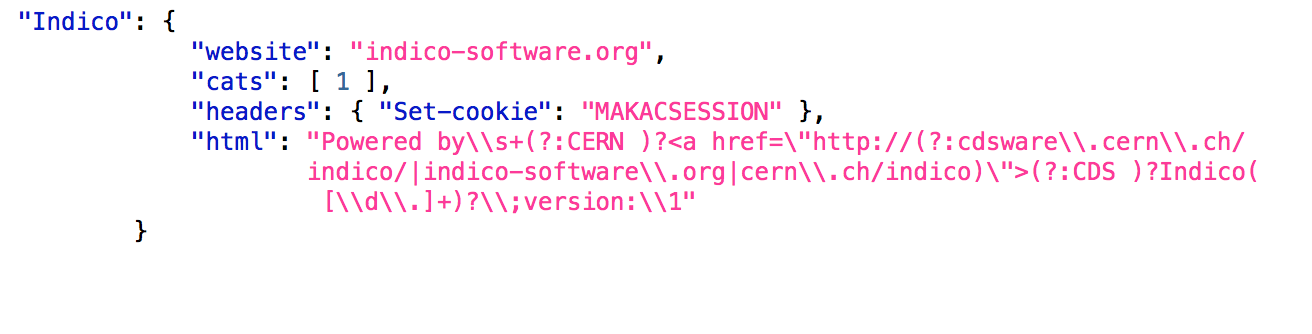
\includegraphics[width=1.0\textwidth]{indico}
  \caption{Indico Detection Rule}
  
\end{figure}
 
\subsection{Detection Scripts}
\paragraph{}
Over the years, CERN Computer Security team has developed individual scripts. Most of these scripts are individual short security tests to check for an emerging vulnerability (e.g. Heartbleed) on CERN resources. Additionally, some scripts detect misconfigurations (e.g. empty landing page) on web servers that could threaten the security of CERN resources. Currently, CERN can detect the following vulnerabilities, using the detection scripts:
\begin{itemize}
\item \textbf{Heartbleed} - The device is vulnerable to OpenSSL Heartbleed vulnerability
\item \textbf{SSL2 Check}: - SSL version 2 is enabled
\item \textbf{SSL3 Check}: - SSL version 3 is enabled
\item \textbf{Weak Cipher} - The server is using a secure cipher
\item \textbf{Homepage Check} - The landing page is empty or the default landing page
\item \textbf{CouchDB Check} - The CouchDB database is protected
\item \textbf{Expired Certificate} - The server is using an expired certificate
\item \textbf{Self-signed Certificate} - The server is using a self-signed certificate
\item \textbf{Non-valid Certificate} - The server is using a certificate that is not valid for the domain
\item \textbf{Non-trusted Certificate} - The server is using a certificate that is not trusted
\item \textbf{Wildcard Certificate} - The server is using a wildcard certificate
\item \textbf{Basic HTTP Authentication} - The website or web server is using Basic HTTP Authentication
\item \textbf{OpenSSL CCS Injection} - The device is vulnerable to OpenSSL Change Cipher Spec (CCS) injection vulnerability

\end{itemize}



\section{Objectives}
\paragraph{}
The main objective of this project is to automate -as much as possible- the procedures for detecting vulnerable web applications. We would like to take advantage of publicly available vulnerability sources, to detect CERN resources that use vulnerable third party products. Another objective of the project is to facilitate scanning CERN resources for critical vulnerabilities in emergency cases, specially when a vulnerability is not specific to a certain, detectable product. This project focuses on detection of vulnerable web applications remotely and when a new vulnerability emerges.

























